\chapter{Kernel Density Estimation}
\label{Kernel Density}

\section{Introduction}
Suppose we have some low dimensional data (1 or 2 variables). How do we start exploring them? Usually, one of the first steps is to plot their histogram to get a feeling of how they are distributed. Histograms are nice because they provide a fast and unambiguous way to visualize our data's probability distribution. However, they are discrete, and sometimes it is useful to have a smooth estimation of the underlying probability density function (PDF) at hand. Figure~\ref{fig:kde_example} shows an example of Kernel density estimate.

\pythoncodenon{code/kde_example.py}

\begin{figure}[htb]
\centering
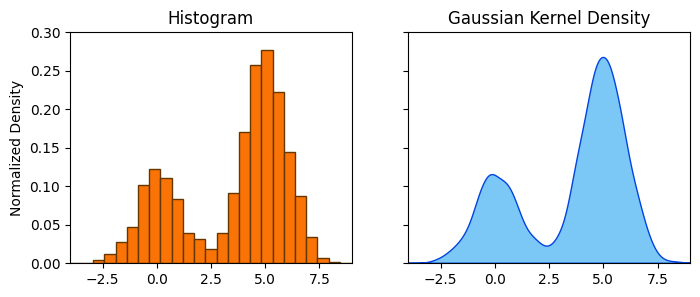
\includegraphics[width=0.75\textwidth]{figures/kde_example}
\caption{Left plot shows an histogram with a sampled distribution. Right plot the Gaussian kernal density estimate.}
\label{fig:kde_example}
\end{figure}

There are two ways to get a smooth PDF from your data.

The \emph{parametric} probability density estimation where we pick a common distribution (say a normal distribution), and we estimate its parameters (e.g., mean, standard deviation) from the data sample.
The \emph{nonparametric} probability such as kernel density estimation (KDE), that we will be discussing today.

\section{The Case of 1 Variable}
In the univariate case KDE is very straightforward. Here is how we'd do it. Assuming we have a set of $N$ samples $x_i=\{x_1,x_2,\ldots,x_N\}$, the KDE, $\hat{f}$, of the PDF is defined as:

\begin{equation}
\hat{f}(x,h)=\cfrac{1}{N}\sum_{i=1}^{N}K_h(x-x_i)
\end{equation}

Basically, in the kernel density estimation approach, we center a smooth scaled kernel function at each data point and then take their average. One of the most common kernels is the \emph{Gaussian kernel}:
\begin{equation}
K(u)=\cfrac{1}{\sqrt{2\pi}}\exp\left(-\cfrac{u^2}{2}\right)
\end{equation}

The $K_h$ is the scaled version of the kernel, i.e., $K_h(u)=\frac{1}{h}K(\frac{u}{h})$. The parameter $h$ of the kernel is called the \emph{bandwidth}, and this little number is a very critical determinant of our estimate's quality. As important as the kernel choice itself! By tweaking its value, we change the width of the kernel.

Kernel density estimation has two main difficulties:
\begin{enumerate}
\item optimal bandwidth estimation;
\item the varying data density makes regions of high data density requiring small bandwidths, and areas with sparse data needing large bandwidths.
\end{enumerate}

Here is a concrete example that sums all of the above assuming a trivial sample $X=\{1,2,3,4,7,9\}$.
And this is the corresponding output:

\begin{equation}
\hat{f}(x, 1)=\cfrac{1}{6}\left(
  \cfrac{e^{-\frac{1}{2}(x-9)^2}}{\sqrt{2\pi}}+
  \cfrac{e^{-\frac{1}{2}(x-7)^2}}{\sqrt{2\pi}}+
  \cfrac{e^{-\frac{1}{2}(x-4)^2}}{\sqrt{2\pi}}+
  \cfrac{e^{-\frac{1}{2}(x-3)^2}}{\sqrt{2\pi}}+
  \cfrac{e^{-\frac{1}{2}(x-2)^2}}{\sqrt{2\pi}}+
  \cfrac{e^{-\frac{1}{2}(x-1)^2}}{\sqrt{2\pi}}\right)
\end{equation}

The following implementation is based on the \texttt{sklearn.neighbors.KernelDensity} utility available in \texttt{python}.

\pythoncodenon{code/kde_one_variable.py}

In Figure~\ref{fig:kde_one_variable}, we plot both the individual Gaussian kernels, along with the kernel density estimate. The black dots are our data points and notice how they are at the kernels' center.

\begin{figure}[htb]
\centering
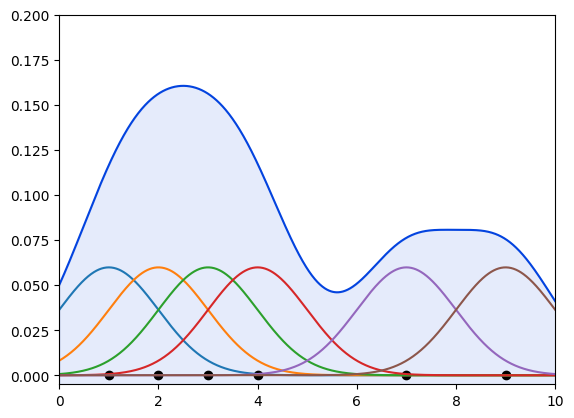
\includegraphics[width=0.75\textwidth]{figures/kde_one_variable}
\caption{In the plot are reported both the individual Gaussian kernels, along with the kernel density estimate for our sample. The black dots are our data points; notice how they are at the kernels' center.}
\label{fig:kde_one_variable}
\end{figure}

In Figure~\ref{fig:kde_bandwidth} the output of our own kernel density estimation for varying values of the bandwidth parameter $h$ is shown. The black dots at the bottom represent our sample data. Notice how for small values of the bandwidth parameter $h$, the KDE is rigged. But, as $h$ increases, the estimate gets smoother and smoother. The selection of the parameter $h$ is, as we have already said, very crucial.

\pythoncodenon{code/kde_bandwidth.py}

\begin{figure}[htb]
\centering
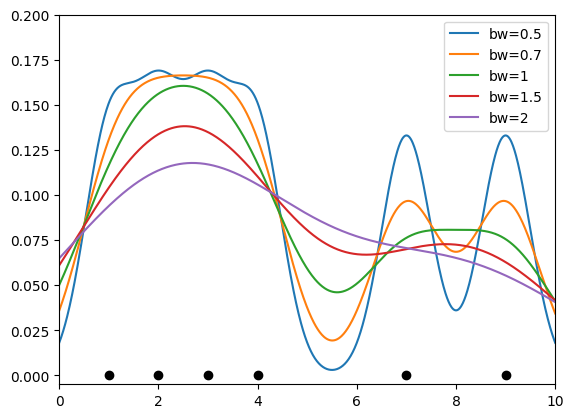
\includegraphics[width=0.75\textwidth]{figures/kde_bandwidth}
\caption{The plot shows how changing the bandwidth parameter affects the density estimate. For small values of $h$ the KDE is rigged. But, as it increases, the estimate gets smoother and smoother.}
\label{fig:kde_bandwidth}
\end{figure}

\subsection{Bandwidth Selection}

There are a number of ways to choose a bandwidth. \emph{Cross validation} is one, but for a much faster approach there are some rules of thumb you can refer to:
\begin{itemize}
\item Scott's Rule: $n^{-\frac{1}{d + 4}}$;
\item Silverman's Rule: $\left(\cfrac{n \cdot (d + 2)}{4}\right)^{-\frac{1}{d + 4}}$.
\end{itemize}

In both of these, $d$ is the dimensionality of your data, and $n$ is the number of data points you have. 
In our example the suggested bandwidth according to Silverman's rule should be 0.74.

\section{Other Kernels}

In principle, we could use whatever kernel we'd like, as long as it is symmetric, non-negative, and integrates to 1. However, our choice should take into consideration the underlying process that generates our data. In the following example, we use a \emph{cosine kernel} on the same data as before.

In Figure~\ref{fig:kde_cosine_kernel} our kernel density estimation for varying bandwidth parameter values $h$ using the cosine kernel.

\pythoncodenon{code/kde_cosine_kernel.py}

\begin{figure}[htb]
\centering
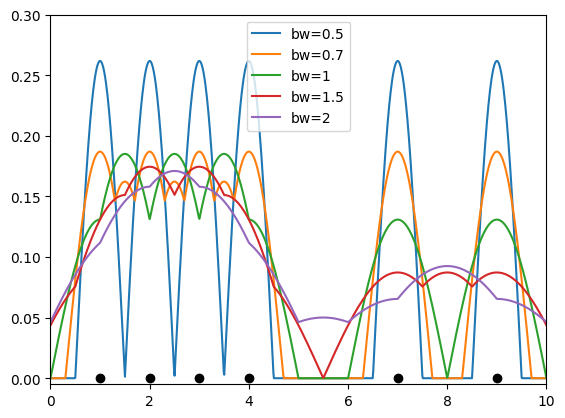
\includegraphics[width=0.75\textwidth]{figures/kde_cosine_kernel}
\caption{The plot shows how changing the bandwidth parameter affects the density estimate. For small values of $h$ the KDE is rigged. But, as it increases, the estimate gets smoother and smoother.}
\label{fig:kde_cosine_kernel}
\end{figure}

\section{KDE and S\&P500}

In this example we attempt to use Kernel Density Estimation techniques to generate a PDF, and then estimate how likely the stock market is to crash from a day to day basis.

So as a first step let's 500 price data (daily OHLC: Open-High-Low-Close) data into a Pandas dataframe
(I have saved in a csv file \href{https://raw.githubusercontent.com/matteosan1/finance_course/refs/heads/develop/input_files/SPX.csv}{SPY.csv}). 
Since we are trying to model the S\&P 500 daily returns, instead of the actual prices, we will use the super-handy \texttt{pct\_change()} function, and put the daily return data into a new column: 'pct\_change'.

It is always good practice to split your data into "training" and "test" sets. Let's say as we use 2009 to 2015's data as the training set, and anything that is 2016 onwards will be used as the test set.

\pythoncodenon{code/kde_spy.py}
\begin{ioutput}
2009-01-05 00:00:00 2015-12-31 00:00:00 2016-01-04 00:00:00 2024-09-24 00:00:00
\end{ioutput}

\begin{figure}[htb]
\centering
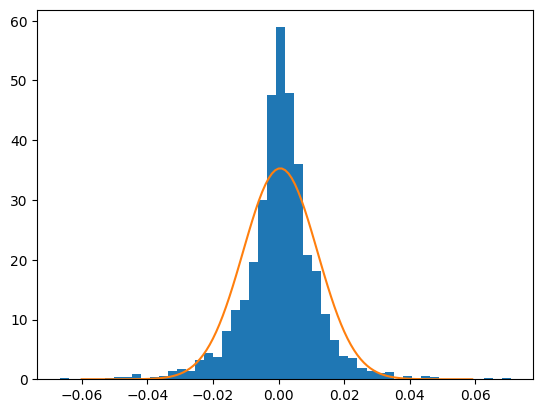
\includegraphics[width=0.7\textwidth]{figures/spy_distro}
\caption{Distribution of the S\&P 500 daily returns in the period 2009-2015.}
\label{fig:spy_distro}
\end{figure}

The histogram in Fig.~\ref{fig:spy_distro} looks like a mal-nourished normal distribution, looks too skinny. Although there are numerical techniques to determine how well (or bad) a PDF matches a distribution we settle for the by eye comparison.

\subsection{KDE Application}

To get a better estimate of the PDF we will be approaching the problem via Kernel Density Estimation. 
Our train\_returns is an 1D-array, meaning it has a shape of (rows,). However most sklearn functions require the data to be re-shaped to have 1 column, i.e. the shape needs to be (rows,1).

Next, the kde variable is loaded up with the Kernel Density object, then fitted with the \texttt{train\_returns\_arr} data.

You may notice that I specified the bandwidth parameter as 0.001. That is just my "guestimate" of a reasonable bandwidth value. Guestimating the bandwidth value is more art than science: if you do not get it right the first time, just change to another value and see if it improves. Feel free to experiment with other numbers for the bandwidth parameter - we will be optimizing this parameter later.

Now, \texttt{kde} is already fitted with the S\&P 500 daily returns data; this means it is a PDF on its own.
We can get the actual probabilities (log-probabilities in this case) values through the \texttt{KernelDensity.score\_samples()} function. Then calculating the actual PDF values is quite straight forward: just calculate the exponential values. Figure~\ref{fig:kde_kde_spy} shows the result.

\pythoncodenon{code/kde_kde_spy.py}

\begin{figure}[htb]
\centering
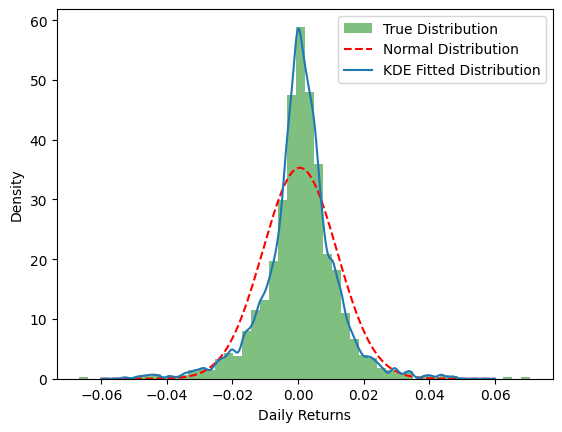
\includegraphics[width=0.75\textwidth]{figures/kde_kde_spy}
\caption{Distribution of the S\&P 500 daily returns in the period 2009-2015 with the KDE PDF.}
\label{fig:kde_kde_spy}
\end{figure}

The KDE Fitted Distribution PDF fits the True Distribution data much better compared to the Normal Distribution curve, i.e. it follows the shape of the True Distribution.

Unfortunately if you zoom into the tails, e.g. -0.02 to -0.06 or 0.02 to 0.06, you can see that the KDE fitted PDF overfits to the True Distribution. To illustrate what I mean, I re-produced the same chart below, but zoomed into one of the tails.

From Fig.~\ref{fig:kde_kde_spy_zoomed} we can see that the KDE Fitted Distribution curve was fooled by the random noise in the True Distribution data. It looks nothing like a "fat tail" distribution.

\begin{figure}[htb]
\centering
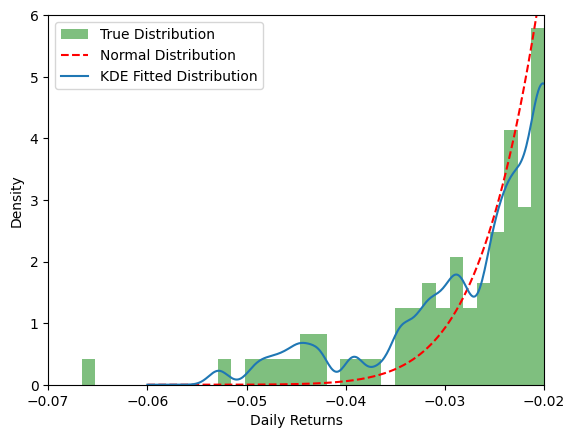
\includegraphics[width=0.75\textwidth]{figures/kde_kde_spy_zoomed}
\caption{Distribution of the S\&P 500 daily returns in the period 2009-2015 with the KDE PDF, zoomed on a tail.}
\label{fig:kde_kde_spy_zoomed}
\end{figure}

\subsection{Optimize the \texttt{KernelDensity} Object}

Luckily \texttt{sklearn} provides the \texttt{GridSearchCV} function: this can help us fine-tuning the \texttt{KernelDensity} parameters so that it generalize better to the noisy data.

\begin{finmarkets}
If you are not familiar with the \texttt{GridSearchCV} function, here is how you work with it: define a "parameter grid" that you want to optimize as a dictionary, for example:

\begin{ipythonbox}
# optimize bandwidth
params = {'bandwidth' : np.linspace(-0.0001, 0.01, 50)}    
                                                           # OR
# optimize bandwidth and kernel type
params = {
    'bandwidth' : np.linspace(-0.0001, 0.01, 30),
    'kernel': ['gaussian', 'epanechnikov', 'exponential']
         }
\end{ipythonbox}
Then run the function, like this:
\begin{ipythonbox}
grid = GridSearchCV(KernelDensity(), 
                    param_grid=params, 
                    cv=20).fit(train_returns_arr)
\end{ipythonbox}                    
Finally read the best parameters via \texttt{grid.best\_params\_}.
\end{finmarkets}

So we can optimize the bandwith (the parameter turns out to be 0.00412) and re-fit the distribution, see Fig.~\ref{fig:kde_opt_band}. 

\pythoncodenon{code/kde_opt_band.py}
\begin{ioutput}
{'bandwidth': 0.004122448979591837}
\end{ioutput}

\begin{figure}[htb]
\centering
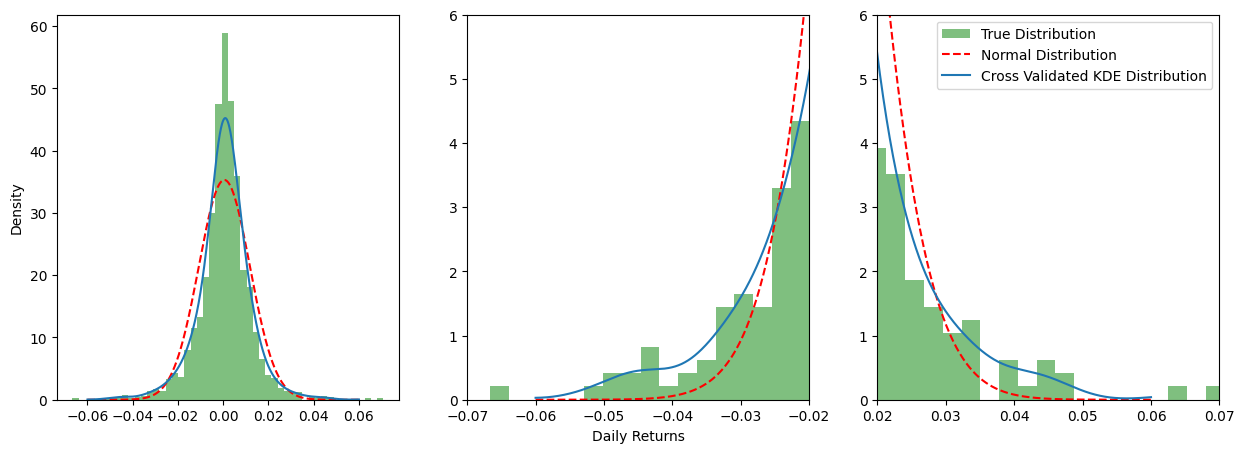
\includegraphics[width=0.9\textwidth]{figures/kde_opt_band}
\caption{Distribution of the S\&P 500 daily returns in the period 2009-2015 with the KDE PDF, zoomed on a tail.}
\label{fig:kde_opt_band}
\end{figure}

Is the optimized KernelDensity any better than before ?
At first glance, the KDE curve looks much better than before. It did not seem to overfit to the random noise at both left and right tails, as you can see by looking at the two right-most plots of Fig.~\ref{fig:kde_opt_band}.

This KDE PDF is by no means perfect, but much better than before.

\subsection{Market Crash Probability}

Let's calculate how likely the stock market will crash more than 4\% a day. Below we are going to use three different methods:
\begin{itemize}
\item using the actual probability, e.g. based on the number of times the S\&P 500 actually crashed more than 4\%;
\item using the optimized KDE's PDF;
\item modelling the stock market returns as a Normal Distribution (which we now know is NOT the right approach).
\end{itemize}

\pythoncodenon{code/kde_market_crash.py}
\begin{ioutput}
Actual probability:              0.568%
Best Fit KDE probability:        0.603%
Normal distribution probability: 0.017%
\end{ioutput}

Within 2009-2015 (our training set's time period), the S\&P 500 crashed (more than 4\%) from a day to day basis, 0.568\% of the time. The best fit (optimized) KDE predicted 0.603\%, not bad at all. But the normal distribution prediction of 0.017% is no where near the reality.

\subsubsection{About Calculating the KDE's Probabilities}

You may have noticed that I calculated the KDE's probabilities using the following:
\begin{ipythonnon}
crash_range = np.linspace(-0.1, -0.04, 1000)
best_kde_probs = np.exp(best_kde.score_samples(crash_range.reshape(-1,1)))
best_kde_probs_integrated = np.trapz(best_kde_probs, x=crash_range)
\end{ipythonnon}

Basically we are trying to calculate the probability of \texttt{train\_returns\_arr} having a value of less than -0.04. That means we need to calculate the probability of it having values between -1.0 and -0.04. This means we are looking for a CDF value:
\begin{equation}
\int_{-\infty}^{-0.04} KDE(x) dx
\end{equation}
(the lower limit of -1.0 is because the most the S\&P 500 can drop is dropping to zero, hence the \texttt{pct\_change()} would be -1.0, or -100\%).

The \texttt{KernelDensity} object does not include a CDF function, so we can only estimate its value by approximating the intergration, in this example I used \texttt{np.trapz()} function (trapz means trapezium rule).

In the code above, \texttt{crash\_range} ranges from -10\% to -4\%, instead of from -100\% and -4\%. -10\% is just an arbitarily small enough number that I chose as the lower limit of the integration, as the KDE's PDF would predict 0\% probability for anything smaller than -0.10 anyway.
